\documentclass[tikz]{standalone}

% \usepackage{newtxtext,newtxmath}

%!TEX root = main.tex

% mytikzset
\usepackage{tikz}
\usetikzlibrary{positioning,arrows,shapes,patterns}
\usetikzlibrary{decorations.pathmorphing}
\usetikzlibrary{decorations.markings}
\usetikzlibrary{decorations.pathreplacing}
\usetikzlibrary{calc}
\usetikzlibrary{patterns}
\usetikzlibrary{decorations.markings}
\usetikzlibrary{petri}

\tikzset{
  vector/.style={thick,double,draw=black, postaction={decorate},
    decoration={markings,mark=at position .6 with {\arrow[black,scale=0.4]{triangle 45}}}},
  axial/.style={thick,double,densely dashed,draw=black, postaction={decorate},
    decoration={markings,mark=at position .6 with {\arrow[black,scale=0.4]{triangle 45}}}},
  gluon/.style={decorate, draw=black,
    decoration={coil,aspect=0.3,segment length=5pt,amplitude=3pt}},
  pseudo/.style={thick, dashed, draw=black, postaction={decorate},
    decoration={markings,mark=at position .6 with {\arrow[red,scale=0.5]{triangle 45}}}},
  scalar/.style={thick,draw=black, postaction={decorate},
    decoration={markings,mark=at position .6 with {\arrow[black,scale=0.5]{triangle 45}}}},
  cut/.style={draw=black, decorate, decoration={snake, segment length=1mm, amplitude=0.2mm}}
}


\definecolor{cola}{rgb}{0.9,0.62,0.0}
\definecolor{colb}{rgb}{0.337, 0.706, 0.914 }
\definecolor{colc}{rgb}{0.0, 0.62, 0.451}

\begin{document}
\nopagecolor
  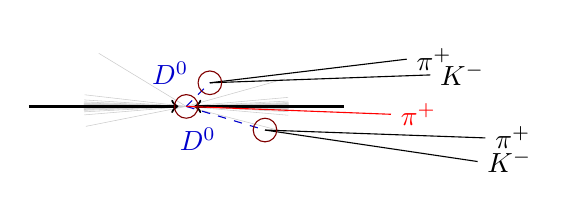
\begin{tikzpicture}[node distance=0.9cm and 1.3cm, baseline=1cm]
%
    \foreach \a in {-10,-8.67,...,10} :
      \draw[very thin, black!20!white] (0, 0) -- ({10/\a}:1.3)  ;
    \foreach \a in {-10,-8.79,...,10} :
      \draw[very thin, black!20!white] (0, 0) -- ({180+10/\a}:1.3);
%
    \draw[->,thick] (-2, 0) -- (-0.1, 0);
    \draw[->,thick] ( 2, 0) -- (0.1 ,0);
%
    \node[coordinate] (vLb) at (0.3 ,0.3) {};
    \draw[blue!80!black,dashed]   ( 0, 0) -- node[above left] {$D^0$} (vLb);
    \draw[] (vLb) -- ++(2.5, 0.3) node[right] {$\pi^+$};
    \draw[] (vLb) -- ++(2.8, 0.1) node[right] {$K^-$};

    \node[coordinate] (vLb2) at (1. ,-0.3) {};
    \draw[blue!80!black,dashed]   ( 0, 0) -- node[below left] {$D^0$} (vLb2);
    \draw[] (vLb2) -- ++(2.8, -0.1) node[right] {$\pi^+$};
    \draw[] (vLb2) -- ++(2.7, -0.4) node[right] {$K^-$};
%
    \draw[red]  ( 0, 0) -- ++(2.6, -0.1) node[right] {$\pi^+$};
    % \node[draw, star,star points=4, fill=white] at (vLb) {};
    \draw[red!50!black] (vLb) circle (1.5mm);
    \draw[red!50!black] (vLb2) circle (1.5mm);
    \draw[red!50!black] (0,0) circle (1.5mm);
  \end{tikzpicture}
\end{document}
